\section{Testing Methodologies}\label{sec:methodology}

We describe two experiments testing OpenCL configurations using our approach. The first is a direct comparison of our approach to CLSmith, the current state-of-the-art in OpenCL test case generation. The second is results from unstructured, opportunistic testing of OpenCL implementations using CLgen, resulting in XX bug reports.

\begin{figure}
  \centering %
  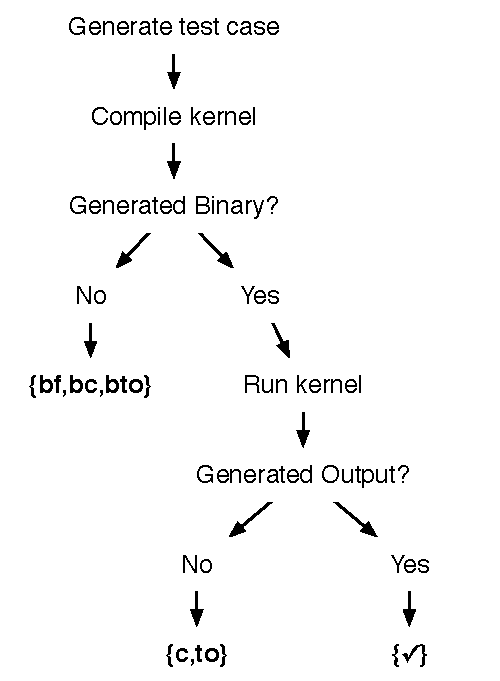
\includegraphics[width=\columnwidth]{img/test_process}%
  \caption{%
  	Test case execution, and possible outcomes. For each test case, a $(+,-)$ pair of outcomes is produced.%
  }%
  \label{fig:test-process} %
\end{figure}



% \subsection{Parameters}
% \begin{table}[t!]
  \scriptsize %
  \centering %
  \rowcolors{2}{white}{gray!25}
  \begin{tabular}{rlll}
\toprule
 Dataset Size &   Global size &  Local size & Optimizations \\
\midrule
          256 &     (1, 1, 1) &   (1, 1, 1) &           off \\
          256 &     (1, 1, 1) &   (1, 1, 1) &            on \\
         4096 &  (128, 16, 1) &  (32, 1, 1) &           off \\
         4096 &  (128, 16, 1) &  (32, 1, 1) &            on \\
\bottomrule
\end{tabular}

  \caption{Test case parameters.}
  \label{tab:cldrive-params}
\end{table}

% Table~\ref{tab:cldrive-params}. 

%\subsection{Classifying test cases}
%
%\cc{Use the results of difftest to determine whether the input sample was formed, well-typed, free from UB, etc. Plot ratio of CLgen and CLSmith outputs according to classifications (CLSmith should be all perfect).}
%
%\begin{enumerate}
%  \item Ill-formed ASCII sequence. The test case contains syntax errors preventing compilation.
%  \item Well-formed program.
%  \item Well-typed program.
%  \item Standard-conformant OpenCL program. The program
%\end{enumerate}

\subsection{Test case execution}

Figure~\ref{fig:test-process} shows the methodology for a single test case.

The possible outcomes for a test case are a build failure (\textbf{bf}), build crash (\textbf{bc}), runtime crash (\textbf{c}), or pass (\textbf{\cmark}). A \textbf{bf} occurs when compilation of a kernel fails, usually accompanied by an error message. A \textbf{bc} outcome on the other hand represents a compiler crash which 

In~\cite{Lidbury2015a}, the authors do not distinguish between compiler crashes and other runtime crashes.

\paragraph{Floating points} The OpenCL 1.2 specification permits acceptable error bounds (ULP) for floating point operations and builtin functions. Some operations like addition, subtraction, and multiplication are precise; divide permits a small error, and builtins vary widely. Thus two implementation may give different answers that both fit within the allowed ranges (and because errors propagate through operations it's hard to even describe the ULP on the final output). \texttt{half\_} functions permit large error bounds. \texttt{native\_} functions have ``implementation defined'' error bounds. TODO: Denormal numbers may optionally be pushed to zero.

CSmith, and by extension, CLSmith, do not support floating point operations. In our observations with testing using CLSmith, we observed that in cases of wrong-code bugs, the computed values are usually entirely incorrect, not only marginally different. We hypothesized that by allowing for relaxed comparisons between floating point values, we could still differential test. We permit a margin of deviation for floating point comparisons. This means that if a compiler were to emit wrong code which changes the computed value only subtly, we may miss it; though we have no reason to suggest that such a case is any more likely than a wrong code bug leading the compiler to produce exactly the same output.
% Section 7.4 of OpenCL 1.2 spec.


\subsection{Classifying test outcomes}

In~\cite{Lidbury2015a}, a configuration is determined to have produced a wrong code result for a kernel if there is a majority of at least 3 among the non-\{\textbf{bf},\textbf{c},\textbf{to}\} results for the kernel, and the configuration yields a non-\{\textbf{bf},\textbf{c},\textbf{to}\} result that disagrees with the majority.

We select the mode output across a range of devices. Voting is used to select the oracle output.
%
\begin{enumerate}
	\item \emph{Wrong code} Program terminates gracefully, but computes a result which differs from the majority.
	\item \emph{Build failure} Online compilation of OpenCL program fails.
	\item \emph{Runtime failure} One or more OpenCL API calls return an error status during the program execution, or the program crashes.
	\item \emph{Okay} Program terminates gracefully and computes a result which agrees with the majority.
\end{enumerate}
